% CS 217A/B, Winter/Spring 2017
% Professor Lixia Zhang
% Project Final Report

\documentclass{sig-alternate}

% General packages and setup
\PassOptionsToPackage{hyphens}{url}\usepackage{hyperref}  % For embedding clickable links to citations
\paperheight=11in
\renewcommand\_{\textunderscore\allowbreak}  % Allows line breaks on words with underscores

\usepackage{listings}

\begin{document}
	
\title{ndnMouse\\Secure Control Interface for a PC Using a Mobile Device}
\subtitle{CS 217B Project Final Report, Spring 2017}
\numberofauthors{1}
\author{
	Wesley Minner\\
	Computer Science M.S. Student\\
	wesleyminner@gmail.com
}

\date{18 May 2017}
\maketitle

% ==============================================================================
\begin{abstract}
This report outlines the results of my efforts on ndnMouse, my class project for CS 217B, as well as my Master's Capstone project. It is open-sourced on \href{https://github.com/wminner/ndnMouse}{Github} under the GNU public license, and available on the \href{https://play.google.com/store/apps/details?id=edu.ucla.cs.ndnmouse}{Google Play App Store}. The goal of ndnMouse is to securely and efficiently control one or more personal computers via remote mouse movement and rudimentary keyboard commands from your phone, running the communication protocol over Named Data Networking (NDN)~\cite{ndn}. In order to compare the design and performance benefits of NDN, ndnMouse also supports communication over UDP. Implementation of both protocols resulted in fairly unique server and clients designs. The pros and cons of each will be explored in this report.

Section 1 will review the features and use cases of ndnMouse, with more detail of the command protocol in Section 2. Details on the security features will be given in section 3, with challenges and trade-offs I have overcome listed in section 4. Performance analysis comparing NDN and UDP implementations is in section 5. Section 6 explores extensions and future use cases for ndnMouse, and section 7 looks at a few of the related works. Finally section 8 concludes this report. Additionally screenshots of the application are in section 7, the Appendix.
\end{abstract}

\keywords{NDN, Mouse, Keyboard, Remote Access, Security}

% ==============================================================================
\section{Overview}
NdnMouse provides remote access to the mouse and keyboard of a PC in order to provide a simple and convenient way to wirelessly interface with your computer. The main use case was to support wireless slideshow/powerpoint control, removing the need for a proprietary piece of hardware (such as a USB clicker device). Anecdotal evidence suggests that users of these devices encounter a variety of issues such as: drained batteries, poor connection, and general hardware failure. Additionally a presenter must also carry around the clicker hardware, which has no other than slideshow control. NdnMouse removes the need for a specialized clicker and adds remote slideshow control to something most people already carry around in their pockets, a smart phone. 

By taking advantage of the local WiFi access point or the phone's WiFi hotspot feature, a user can use their Android smart phone as a virtual touchpad and simple keyboard, providing the functionality needed to step through a powerpoint presentation without any additional hardware. NdnMouse also may be of use during times of hardware failure, providing an emergency backup mouse or keyboard when the user has limited options to interface with their PC.

Both NDN and UDP/IP transport/routing protocols are supported, encrypting packets with AES if a password is provided by the user. Additionally NDN can provide some extra features in the form of interest (query) condensing, allowing the phone server to better scale its performance when multiple PC clients are connected. More on this idea will be described in Section 5. However the protocol choice should ideally be transparent to the user, as all features are supported on both NDN and UDP.

\subsection{Features}
NdnMouse supports full mouse control: relative cursor movement, left click, right click, and a shortcut allowing tap-to-click on the touchpad. Sensitivity and precision settings are also provided, for fine tuning the feel of the movement. Two-finger scrolling works similarly to Apple laptops, with inversion and sensitivity settings as well. Rudimentary keyboard support allows the user to execute common slideshow control commands, such as using the arrow keys or the spacebar to easily change slides. Additionally custom typed messages are supported, allowing the user to type any message using the built-in Android keyboard. Upon sending the message, all receiving client PCs will then virtually the characters out instantly on whatever program window is selected at that time.

The security for ndnMouse was designed to defend against packet snooping, replay attacks, privacy attacks, and brute force attacks. More details will be given in section 3. The user may also choose to not use a password, which sends the communication protocol in cleartext and avoids a minor amount of encryption/decryption overhead. 

\subsection{Supported Platforms}
NdnMouse is composed of two applications: the server/producer Java application (running on the Android phone), and the client/consumer Python application (running on the PC). Any relatively modern Android phone is supported (Android 4.1 and up), and basically any PC that can run NDN's Network Forwarding Daemon (NFD)~\cite{nfd} and Python3~\cite{python3}. Since Python runs on the three major operating systems (Linux, OSX, and Windows), the limiting factor is NFD, which only currently runs on Linux and OSX. However Windows PCs can still use ndnMouse by limiting their protocol choice to UDP only.

Other dependencies include a few Python libraries needed for the PC client, specifically PyAutoGUI~\cite{pyautogui}, PyCrypto~\cite{pycrypto}, and PyNDN~\cite{pyndn}. PyAutoGUI provides mouse and keyboard control, as well as some simple dialog boxes for collecting user input. PyCrypto handles all the cryptography operations, and PyNDN provides the API for using NDN and for interfacing with NFD. The Android application uses jNDN~\cite{jndn} to access the NDN API, but this library comes compiled into ndnMouse's APK and requires no outside installation by the user. Both the PC and Android phone must have NFD installed and running to communicate over NDN.

\section{Protocol}
NdnMouse can run its communication protocol four different ways, depending on the transport protocol used (UDP or NDN) and if a password is provided by the user (security on or off).

\subsection{UDP}
Without a password (all security off), packets are transmitted in cleartext and are at most 16 bytes. UDP uses connection-oriented communication by having the client send an \texttt{OPEN} message to the server, similar to a TCP \texttt{SYN} packet. This asks the server to establish a \textit{session} between the client and itself. An \texttt{OPEN-ACK} reply message is used to respond to the \texttt{OPEN} message and completes the connection setup.

Once a session is established, the server will send unsolicited mouse commands\footnote{I will refer to all commands ndnMouse can send as mouse commands, though this includes supported keyboard commands as well.} to its clients. The data format is not strict across all possible mouse commands, but generally takes the form of one character dictating the type of command, followed by any additional information for that command. For example, a mouse movement command is of the form \texttt{M<x-4B><y-4B>}. I denote the \textit{x} and \textit{y} coordinates each have a fixed length of 4 bytes by appending "\texttt{4B}." See \hyperlink{tab:msgFormat}{Table 1} for the supported, non-secure message formats.

\begin{table}
	\hypertarget{tab:msgFormat}{}
	\begin{center}
		\begin{tabular}{| l | l |}
			\hline
			Message Type & Message Format\\ \hline\hline
			Movement & \texttt{M<x-4B><y-4B>}\\ \hline
			Click & \texttt{C<click\_message>}\\ \hline
			Scroll & \texttt{S<x-4B><y-4B>}\\ \hline
			Keyboard & \texttt{K<keyboard\_message>}\\ \hline
			Typestring & \texttt{T<type\_string-10B-max>}\\ \hline
		\end{tabular}
		\caption{Non-secure message formats}
	\end{center}
\end{table}

Heartbeat messages are sent once every one second to keep the connection alive when no other mouse command packets are being sent. The client query packet contains the message \texttt{HEART}, and the server reply contains the message \texttt{BEAT}. The main goal of heartbeats was to detect when the server had lost its session with the client, such as during a server reset or crash. In these cases, the client would miss a certain number of heartbeat replies from the server, triggering a session restart on the client side. The client would then try to open a new session using \texttt{OPEN} messages. After receiving a \texttt{OPEN-ACK}, the session would resume normal activity.

Lastly a \texttt{CLOSE} message is sent by the client upon exiting the application. This lets the server know that it can stop sending unsolicited mouse command messages. Note that reliable delivery and in-order processing of packets is not needed for ndnMouse, letting the application take advantage of the simplicity and performance of UDP. The simple, connection-oriented communication I implemented on top of UDP allows ndnMouse to gracefully recover from server/client connection problems.

When security features are turned on, the UDP communication protocol becomes slightly more complex to prevent specific types of malicious attacks. Both the packet format and the payload message require changes. In \hyperlink{tab:secureMsgFormat}{Table 2}, the secure message formats are listed. A four byte sequence number is added to the front of each message, and then the entire message will then be encrypted, as described in the section 2.3 on Mouse Packets. The message length is also fixed to 16 bytes, using PKCS5 padding~\cite{rfc8018}.

\begin{table}
	\hypertarget{tab:secureMsgFormat}{}
	\begin{center}
		\begin{tabular}{| l | l |}
			\hline
			Message Type & Secure Message Format\\ \hline\hline
			Movement & \texttt{<seq-4B>M<x-4B><y-4B>}\\ \hline
			Click & \texttt{<seq-4B>C<click\_message>}\\ \hline
			Scroll & \texttt{<seq-4B>S<x-4B><y-4B>}\\ \hline
			Keyboard & \texttt{<seq-4B>K<keyboard\_message>}\\ \hline
			Typestring & \texttt{<seq-4B>T<type\_string-10B-max>}\\ \hline
		\end{tabular}
		\caption{Secure message formats}
	\end{center}
\end{table}

\subsection{NDN}
When designing the NDN communication protocol, I found that the architecture would have to differ significantly from the UDP communication style. The consumer/producer\footnote{For NDN, the consumer can be thought of as the client, and the producer as the server. I may use these terms interchangeably as they are closely related.} relationship encourages the use of a connection communication. In this way, the consumer can easily get the data it requests without worrying about the location, as NDN data packets are immutable and authenticated via a signature. However note that I do not validate the signature on my NDN produced packets. More details on this will be given in section 4.1. ndnMouse's NDN communication protocol also uses the same message formats given in Table 1 and 2. The only difference is how they are retrieved by clients/consumers.

To allow multiple consumers to share the same data packets, I chose to use a connectionless design. This also fit well with the NDN callback-oriented API, where all communication activity on the server/producer is handled by a single main thread, set up beforehand to serve particular named interests. Contrast this to ndnMouse's UDP communication protocol, which spins off worker threads to handle each client separately. There is no need to do this with NDN as the connectionless design lets the producer be consumer agnostic. The NDN producer is set up to serve the interest names given in \hyperlink{tab:ndnInterestNames}{Table 3}. The sequence number and password salt interests are only served when ndnMouse has security turned on.

\begin{table}
	\hypertarget{tab:ndnInterestNames}{}
	\begin{center}
		\begin{tabular}{| l | l |}
			\hline
			 Interest Name & Purpose \\ \hline\hline
			\texttt{/ndnmouse/move/} & Movement Data\\ \hline
			\texttt{/ndnmouse/command/} & Command Data\\ \hline
			\texttt{/ndnmouse/seq} & Sequence Number Sync\\ \hline
			\texttt{/ndnmouse/salt} & Password Salt Data\\ \hline
		\end{tabular}
		\caption{Secure and non-secure NDN served interests}
	\end{center}
\end{table}

While the NDN producer may run a connectionless communication protocol without security, an exception had to be made to support sequence numbers on the secure version. The sequence number primarily helps prevent replay attacks by functioning as a nonce. Each consumer must have some idea of the largest sequence number they have witnessed in returned data from the producer. This means that each consumer must maintain a state and cannot run a completely connectionless communication protocol. More details will be given in the section 3.

\subsection{Mouse Packets}
For non-secure communication, mouse packets are exactly the same as the message formats listed in \hyperlink{tab:msgFormat}{Table 1}. In those cases, the payload is the entire packet. When security is used, then additional information must be carried with the payload, and encryption is performed on select segments of the mouse packet. Specifically a 16 byte initialization vector (IV) is prepended to the front of every message, which will be used with AES encryption. More on this in security section 3. Additionally the total packet length is fixed at 32 bytes, and encryption is only performed on bytes 17-32. See \hyperlink{fig:mousePacketDescription}{Figure 1} for a visual representation of the secure mouse packet.

\begin{figure*}
	\hypertarget{fig:mousePacketDescription}{}
\begin{lstlisting}
                                    1                   2                   3
bit num:        0 1 2 3 4 5 6 7 8 9 0 1 2 3 4 5 6 7 8 9 0 1 2 3 4 5 6 7 8 9 0 1 2
                -----------------------------------------------------------------
contents:       |              IV               |  Seq  |  Message (PKCS5 pad)  |
                -----------------------------------------------------------------
encryption:	|<======== plaintext ==========>|<========= ciphertext ========>|
\end{lstlisting}
\caption{Secure mouse packet description}
\end{figure*}

% ==============================================================================
\section{Security}
Creating a secure communication protocol was one of my top priorities for ndnMouse. Few NDN applications thus far have implemented any meaningful security, and the scope of my project allowed me to spend the time to properly design a secure protocol. There are three major components to the security architecture: data encryption, sequence number validation, and password salting. These components are supported by both the UDP and NDN communication protocols of ndnMouse, though there exists a few minor implementation differences which will be explained below.

\subsection{Data Encryption}
Data encryption is handled by standard AES with cipher block chaining (CBC). CBC requires a new, random IV for each packet to ensure that the first block of a known piece of data always encrypts to a different piece of ciphertext. Remaining blocks in the data (if any) then use the prior block to act as the IV, which creates a chain of block encryptions. I chose this method because the alternative, electronic codebook, is known to be relatively weak for encrypting data with similar or the same payloads. NdnMouse would expect to send many click messages with the same data content, so I did not want these messages to encrypt to the same ciphertext for privacy reasons. 

A 16 byte block size was used for CBC, which meant that packets only contained one block to be encrypted. While this means that CBC provides little benefit to the AES encryption, ndnMouse packet sizes may grow in the future to accommodate more data per packet. Then CBC may be needed to encrypt multiple blocks of data. Additional thoughts on ndnMouse feature extensions are given in section 6.3.

To ensure that the client/consumer can always decrypt a secured packet, the cleartext of the unique IV used for each packet's encryption is prepended to the front of the ciphertext. It is common to transmit IVs in cleartext, as knowledge of the IV alone cannot help decrypt an encrypted piece of data. The IV merely helps the final ciphertext to look more unique, regardless of the underlying cleartext data.

\subsection{Sequence Number Validation}
Even though each secured packet was unique via the IV and AES encryption, a replay attack could be used to maliciously force the client to perform an mouse command. To prevent this, sequence numbers were added to the front of each packet, which could then be validated on both the client and server side before executing any mouse or protocol commands. The sequence number policy of ndnMouse enforces that no command should be executed which contains a sequence number lower than the largest sequence number witnessed by the device. 

Upon opening a new ndnMouse session, the client sends the initial \texttt{OPEN} message with a sequence number of zero, and the server replies with the \texttt{OPEN-ACK} message and a sequence number of one. Thereafter each mouse or protocol command uses the current sequence number incremented by one. Since each sequence number is only used once, this field can be thought of as a nonce. Since ndnMouse uses in-order sequence numbers, it is easy to determine if a number was previously used. So if an attacker recorded a set of encrypted packets and attempted to replay them at a later time to the client, the client would find old sequence numbers and simply ignore the commands.

The question then arises whether packets delivered out-of-order would cause a problem for ndnMouse. This is not the case as both the server and client have a \textit{catch-up} mechanism, which allows them to set their sequence number to any number higher than what they are currently set to. If packets were to arrive with sequence number order 2, 4, and 3, the last packet command would be ignored. The catch-up mechanism would assume that sequence number 3 was lost or delivered late, skipping ahead to a current sequence number of 4. For a latency-sensitive mouse control application, late packets are useless anyway!

\subsection{Password Salting}
Users typically resort to using the same password for a given application. With this in mind, if packets were captured by a malicious subject during a given session of ndnMouse, the decryption key\footnote{For this report, the term \textit{key} refers to a cryptographically hashed user password} would be the same as any future session. Then replay attacks would still be possible \textit{intra}-session\footnote{between two different sessions} (as long as the sequence number was not relatively old). This is different than the prevention of \textit{inter}-session\footnote{within the same session} replay attacks that sequence numbers provided us. To resolve this security hole, random password salts were added to ndnMouse.

For ndnMouse, a password salt is 16 random bytes generated by the client or server, which will be appended to the user password before hashing occurs to generate the key. The UDP communication protocol uses the initial IV on the client's \texttt{OPEN} message to use as the password salt for the remainder of the session\footnote{The UDP \texttt{OPEN} message is encrypted with the unsalted password hash, but there after all other messages will use the salted password hash.}. Like IV's, a password salt may be passed in cleartext as it does not help decrypt an encrypted message or reveal the user password in any way. 

For the NDN communication protocol, all interest names are given in cleartext, so no IV can be used from the client/consumer as the password salt. To resolve this, the server/producer will create a random password salt on session startup. The consumer can simply retrieve this data by sending an interest for \texttt{/ndnmouse/salt} as seen in \hyperlink{tab:ndnInterestNames}{Table 3}. All other data returned for interests will be encrypted using the key generated with the salted user password.

Traditional uses of a password salt are for storing user passwords securely in a database. Passwords are salted, then hashed, with the database only storing the resulting hash and the password salt in cleartext. In this way, a compromised database will not reveal the actual user passwords to the attackers. This would require a significant brute force effort of comparing a password rainbow table using the cleartext salts provided for every user, resulting in a table several magnitudes larger than a rainbow table needed for unsalted passwords. 

NdnMouse does not store any form of the user password in persistent memory. However ndnMouse should not be susceptible to intra-session replay attacks. Therefore by simply using a password salt, each session will have a unique key for encryption/decryption even if the same user password is used. Any replayed packets from previous sessions will not decrypt correctly on the client side, and will be thrown away silently.

\subsection{Attack Types and Defenses}
As stated in the features section, security was designed to defend against packet snooping, replay attacks, privacy attacks, and brute force attacks. Each of the security features mentioned above target one or more of these malicious behaviors. Encryption prevents malicious subjects from snooping data from packets. Replay attacks are prevented both inter-session and intra-session via sequence number validation and the use of password salts respectively. 

The effectiveness of privacy attacks is decreased by using new, random IVs on each individual packet. This prevents two packets with the same data being encrypted to the same ciphertext, reducing the amount of inference an attacker can gain by analyzing the data flow. Finally the efficiency of brute force attacks is limited by using a new password salt for each session. NdnMouse sessions are expected to be relatively short-lived, as slideshow presentations represent the primary use case. As a result, a relatively small amount of packets using the same key will be exposed for a brute force attacker to collect.
	
% ==============================================================================
\section{Challenges and Trade-offs}
NdnMouse's met with several challenges and trade-offs during implementation. Development of ndnMouse's four different protocol styles (UDP or NDN, security on or off) flowed in a serial manner. The UDP server implementation was built first, then ported to NDN. After that, the server classes were extended to support security, first in UDP and then in NDN. It was more challenging that I initially anticipated to port the UDP server to NDN, as the way of thinking for each style of communication differed greatly. UDP took on a traditional worker thread design, while NDN lent itself to a more simple, single-threaded, callback approach. Other challenges included the lack of unsolicited data support in NDN, and my decision to use a shared secret rather than NDN's built-in signature validation.

\subsection{Unsolicited Data}
UDP can easily send unsolicited data through a socket, but NDN cannot send unsolicited data through a face. By design, it must receive an interest packet first. For my application, unsolicited data is useful to send unpredictable mouse commands, like mouse clicks, avoiding the need for continuous polling from the client side. Mouse movement, on the other hand, must be continuously polled at a constant rate, which translates nicely to the NDN interest/data model.

To handle mouse clicks and other commands using NDN, I created a separate interest that would ask the producer for mouse command data at a constant rate. A majority of the packets time out due to no available data, but when the user does execute a mouse click or a special keyboard key-press, the consumer side will still receive the data in a timely manner. Though this method is not as efficient as UDP, the latency is still low enough to be nearly imperceptible by the user.

\subsection{Signature Validation vs Shared Password}
Enforced packet signatures is one of the most important features of NDN, as it allows a consumer to acquire data from any location, independent of where it was originally produced. A consumer can always verify if the data originates from the producer they expect by validating the data's signature. I originally intended to use this method to validate the consumers (PCs) that try to get data from the producer (phone). However due to time constraints and ease-of-use considerations, I eventually decided to forgo this idea for a simpler strategy that relied on a shared user password.

Signature validation presented a complex problem to solve in order to simply trade a shared symmetric key. Since ndnMouse is meant to be set up by the same person on at least two local devices, typing in a simple user password allowed both devices to have the same symmetric key without any additional work. If ndnMouse had to use signature validation to trade a symmetric key, there would then be additional user-workflow problems with deciding who could receive that symmetric key from the producer and who could not. Even with proper NDN certificates installed on each device, the user would likely need to whitelist devices that were allowed to act as consumers for ndnMouse.

By having the user decide the shared secret offline and pass it as a parameter for each controlled device, ndnMouse can provide both consumer authentication and a shared symmetric key for encryption/decryption of data. Also I assume that most users are familiar with how a shared password would work for this type of application. If ndnMouse required a whitelist of authenticated NDN devices, it might burden the user with the need to understand more of NDN's inner workings. 

While these arguments may not full justify stepping away from the ideal NDN workflow (which uses signature validation), I believe that a shared password works best for ndnMouse's use cases and fulfills its ease-of-use goal. However future extensions of ndnMouse may be able to add in a module to collect a shared secret via signature authentication, making use of all the features NDN has to offer.

% ==============================================================================
\section{Performance Analysis}

\subsection{UDP vs NDN}

\subsection{Event Driven Architecture}

\subsection{Stateful Multi-Threaded Architecture}

% ==============================================================================
\section{Extensions}

\subsection{NDN Performance Optimization}

\subsection{Many Mouse, One Computer}

\subsection{Cross-Computer Mouse Support}

% ==============================================================================
\section{Related Works}

% ==============================================================================
\section{Conclusion}

% ==============================================================================
%\section{Expectations}
%My expectations have only slightly changed since my initial project proposal. I plan to focus on the security aspects of NDN, implementing full mouse control with some basic keyboard control (to support remote slide show/powerpoint control). During my security implementation work, I realized that the signature validation capabilities of NDN may not be practical for ndnMouse's purposes. Requiring the user to install certificates and a trust anchor ahead of time for each of their devices is significantly more work than using a simple user-password. Using asymmetric encryption via certificates to securely pass a symmetric encryption key between devices also adds an unneeded extra step to each session setup, which I currently skip by requesting a offline, shared secret from the user in the form of a password. For these reasons I will deprecate the signature validation requirements for ndnMouse and focus on other quality of life enhancements for the user. I may return to signature validation experimentation if I have extra time at the end of the quarter.
%
%I am slightly ahead of my initial timeline projections, but I also plan to finish somewhat early to gain the Capstone faculty signatures required for graduation. If all goes well, there may be at least one week I can use to add additional ease-of-use features, such as two-finger scrolling support. For now I am focusing on the minimum viable product, which includes mouse control, basic keyboard support, and full encryption security.


% ==============================================================================
% Bibliography
\bibliographystyle{abbrv}
\bibliography{sigproc}  % sigproc.bib is the name of the Bibliography in this case

% ==============================================================================
\section{Appendix}
Screenshots of the Android and PC applications follow. The Android app can be downloaded directly from the \href{https://play.google.com/store/apps/details?id=edu.ucla.cs.ndnmouse}{Google Play App Store}, and the PC client application can be downloaded from the \href{https://github.com/wminner/ndnMouse/tree/master/pc_client}{Github} repository.

\begin{figure}[ht]
	\hypertarget{fig:start}{}
	\centering
	\caption{Start screen}
	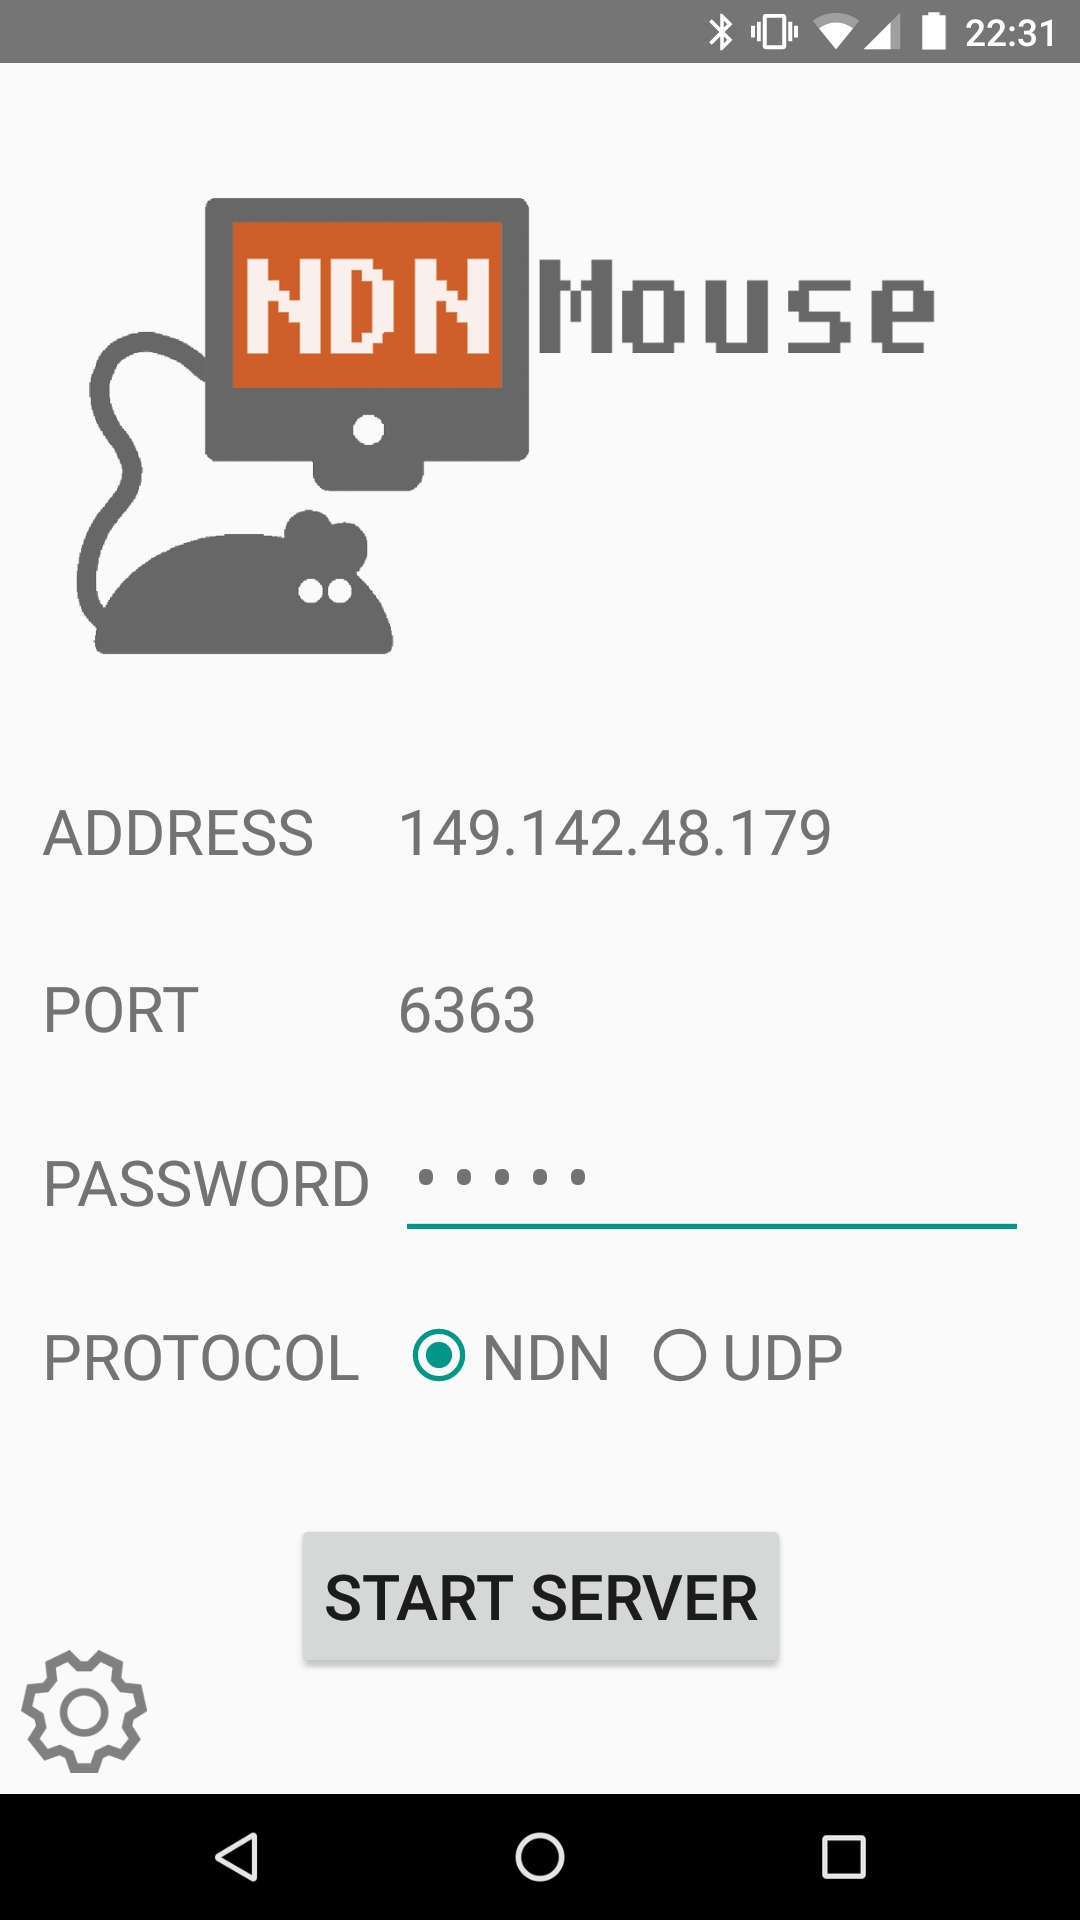
\includegraphics[width=6cm]{screenshots/start}
\end{figure}

\begin{figure}[ht]
	\hypertarget{fig:settings}{}
	\centering
	\caption{Settings screen}
	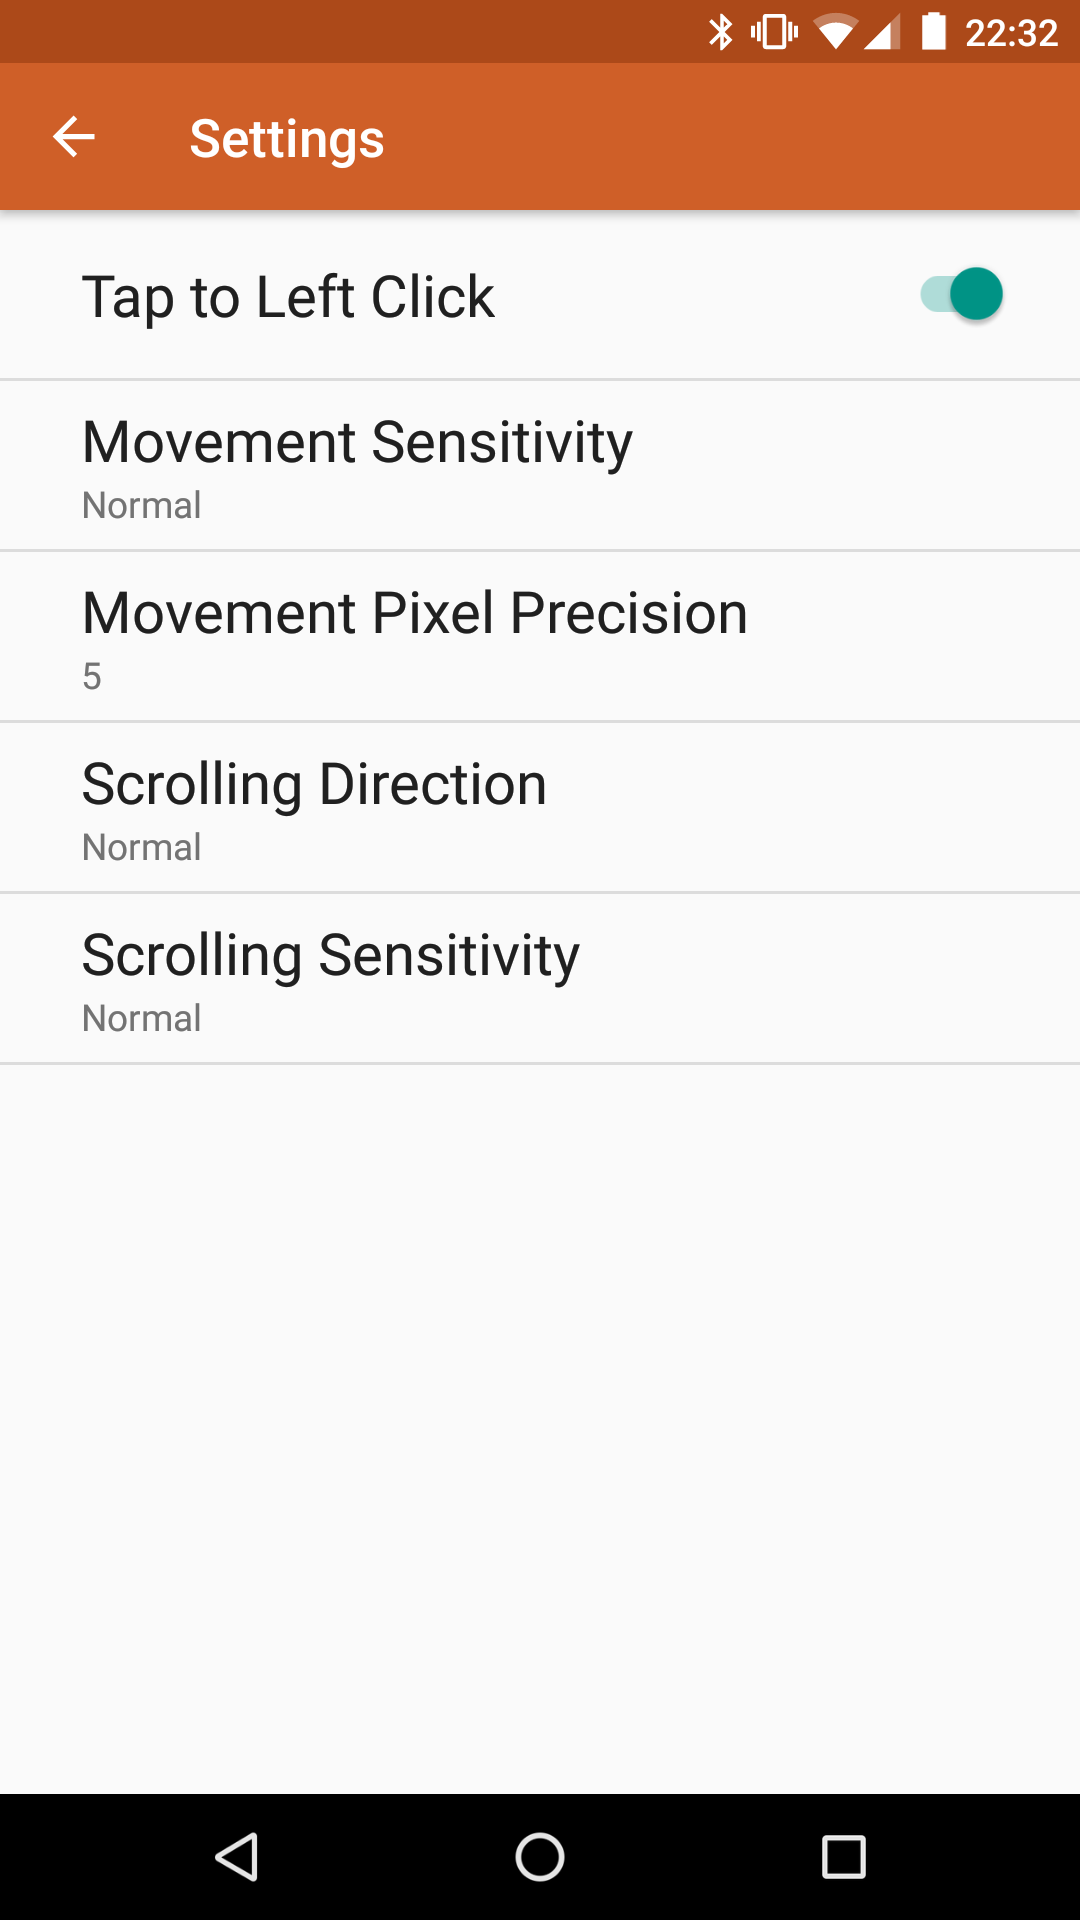
\includegraphics[width=6cm]{screenshots/settings}
\end{figure}

\begin{figure}[ht]
	\hypertarget{fig:touchpad}{}
	\centering
	\caption{Touchpad screen}
	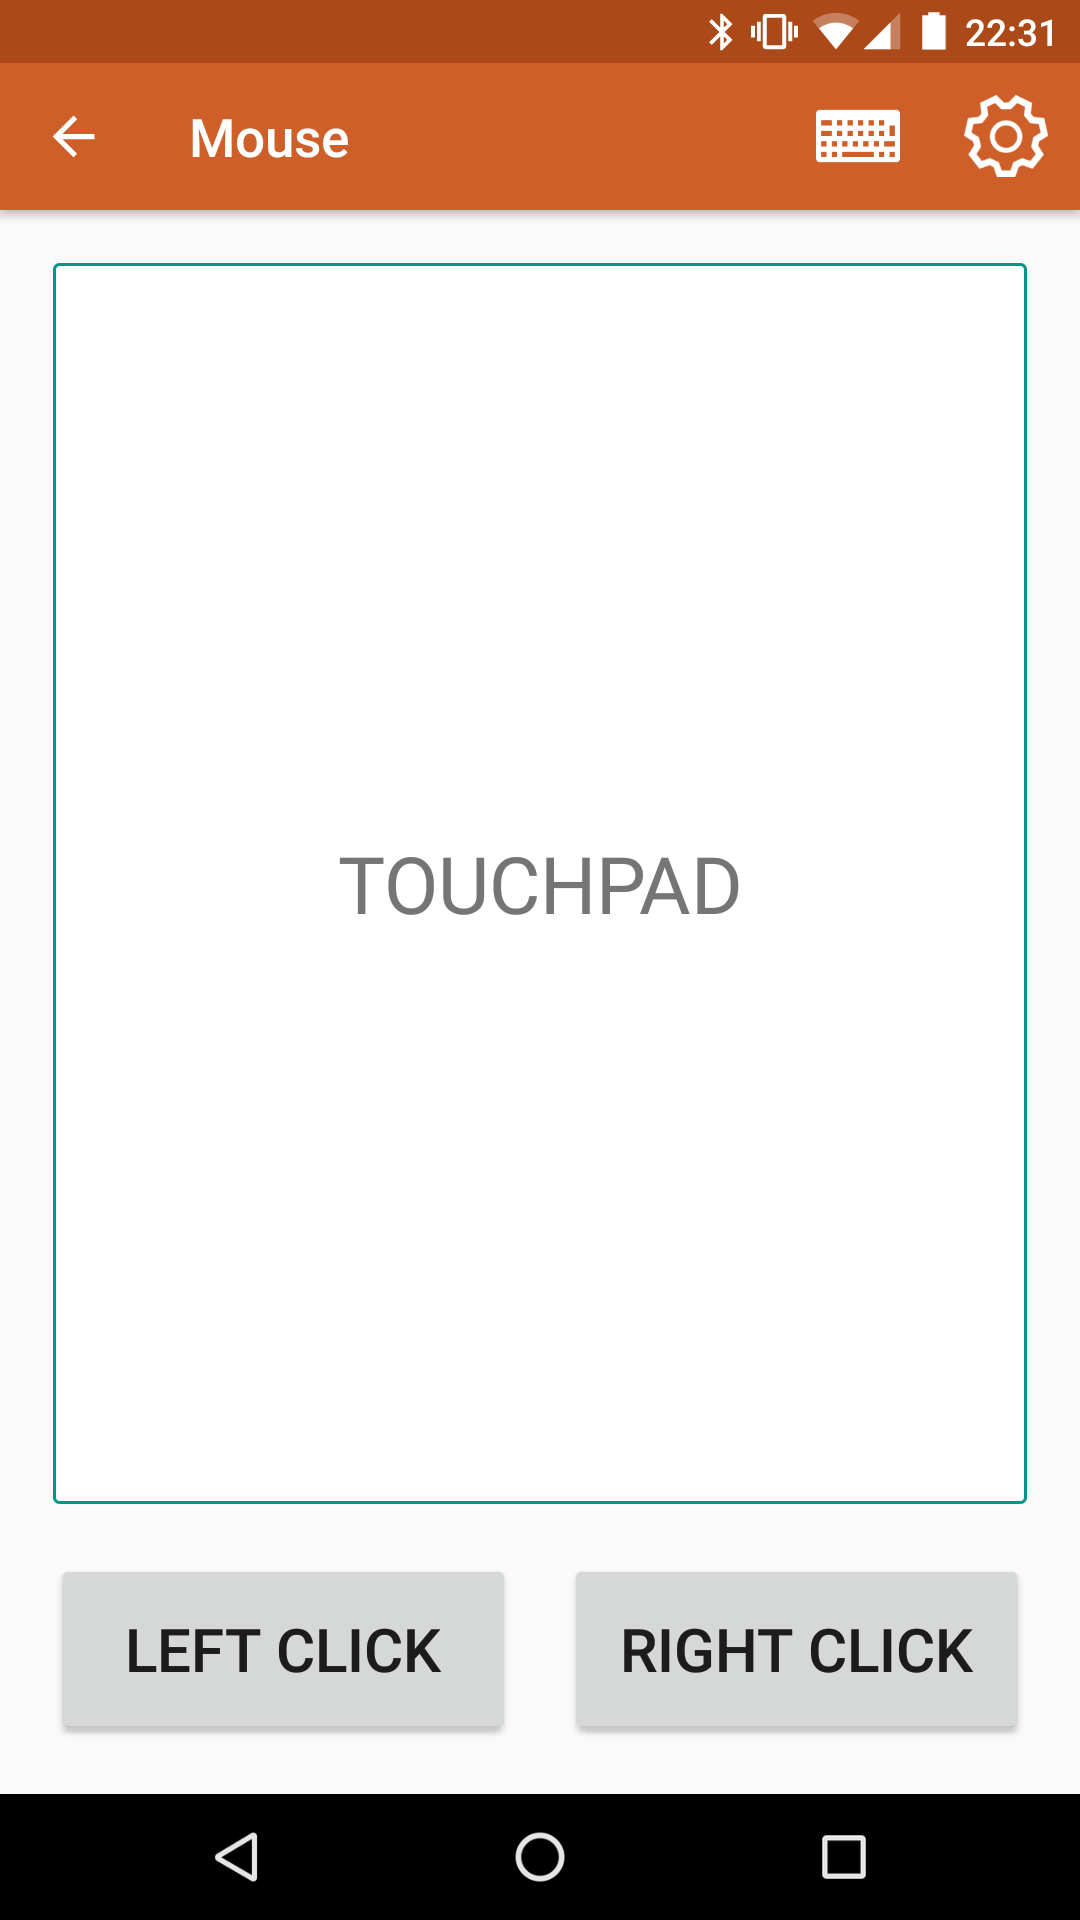
\includegraphics[width=6cm]{screenshots/touchpad}
\end{figure}

\begin{figure}[ht]
	\hypertarget{fig:keyboard}{}
	\centering
	\caption{Keyboard screen}
	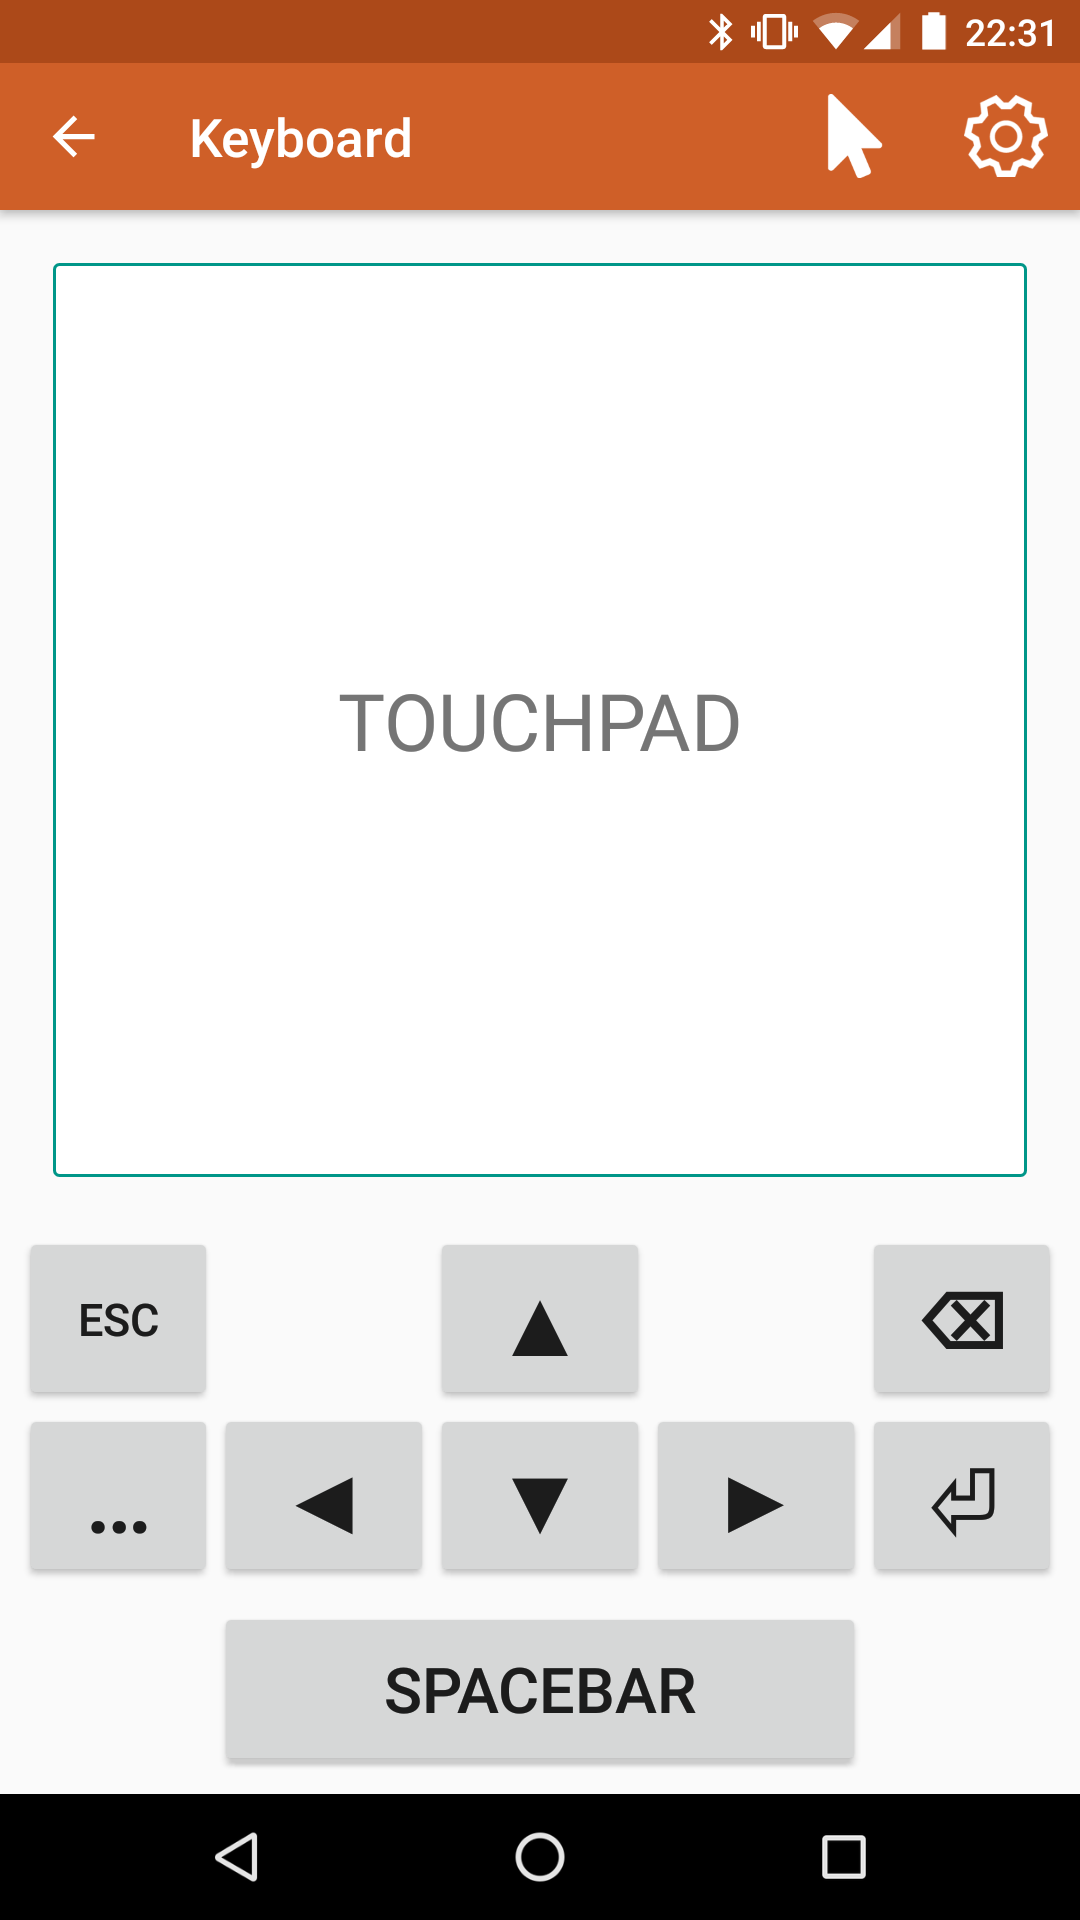
\includegraphics[width=6cm]{screenshots/keyboard}
\end{figure}

\begin{figure}[ht]
	\hypertarget{fig:custom\_type\_message}{}
	\centering
	\caption{Custom typed message entry}
	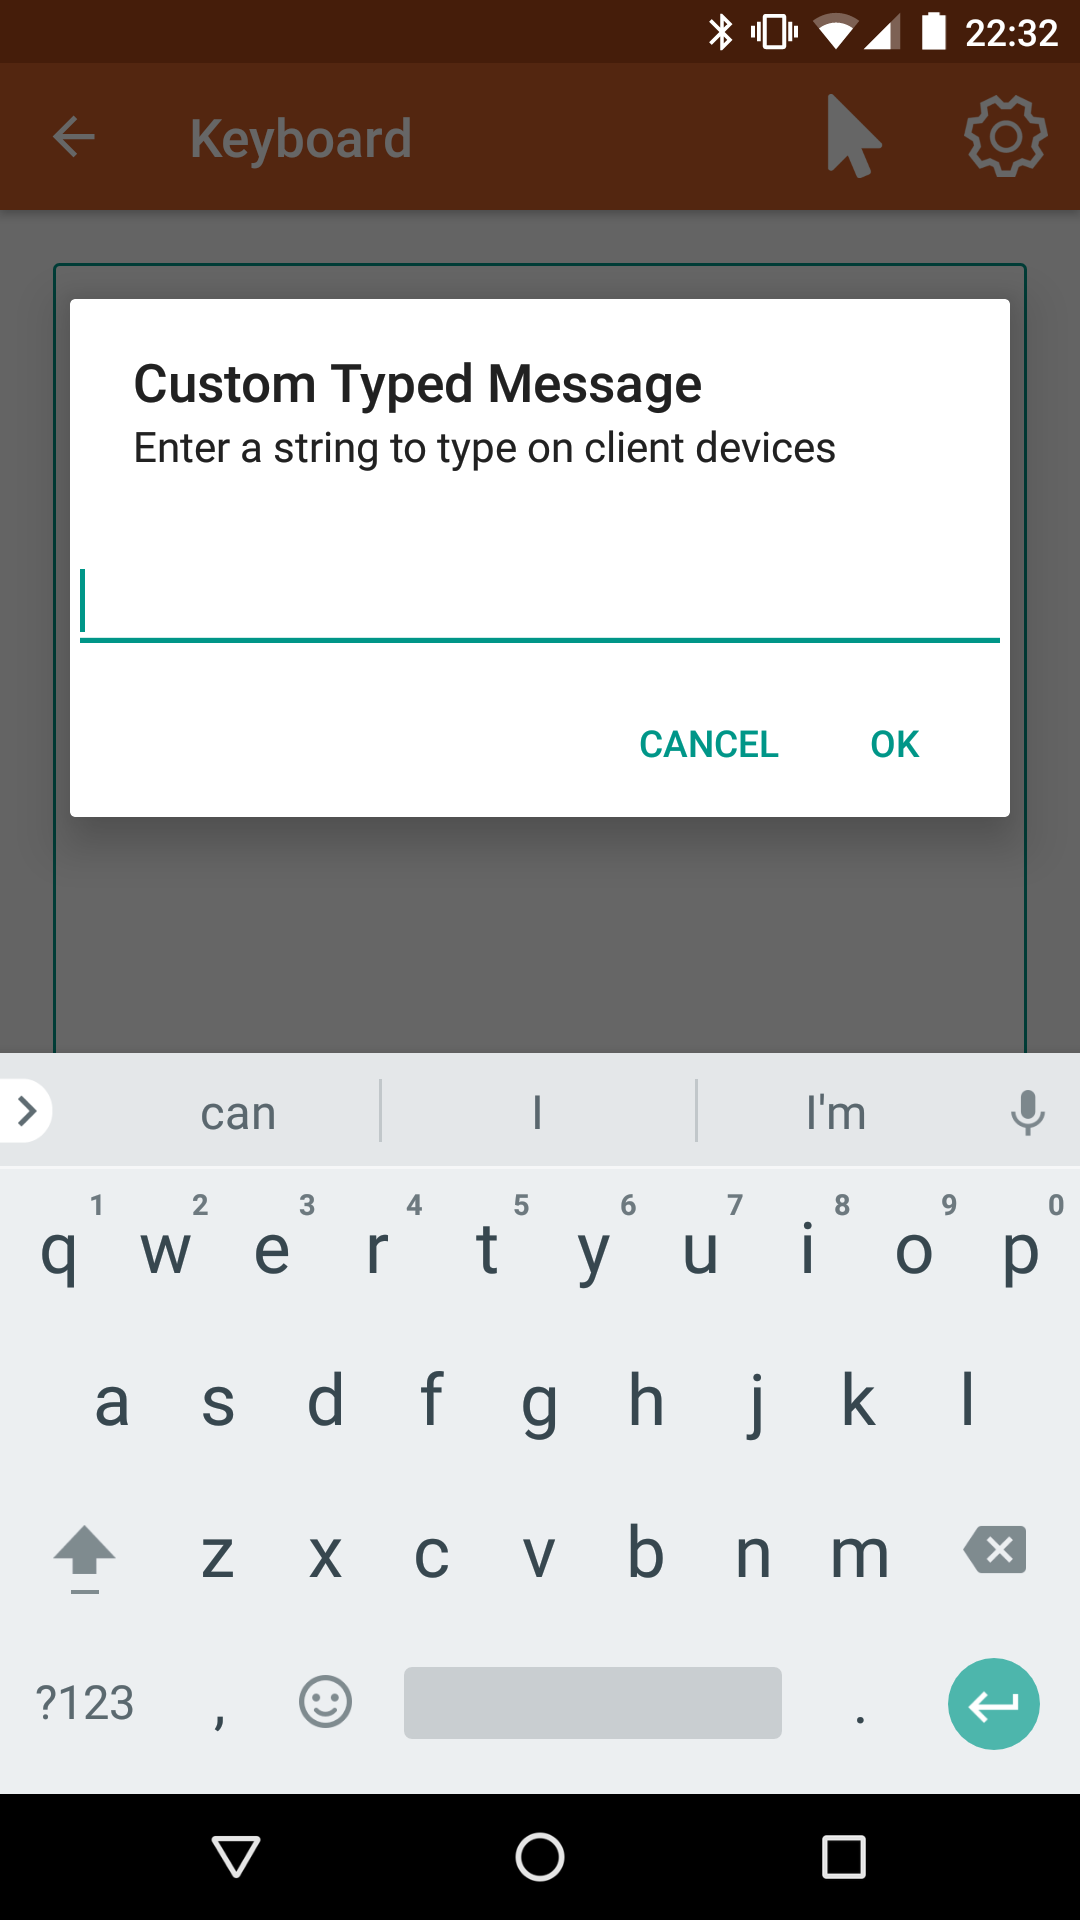
\includegraphics[width=6cm]{screenshots/custom_type_message}
\end{figure}

\begin{figure}[ht]
	\hypertarget{fig:client1}{}
	\centering
	\caption{PC program IP address entry}
	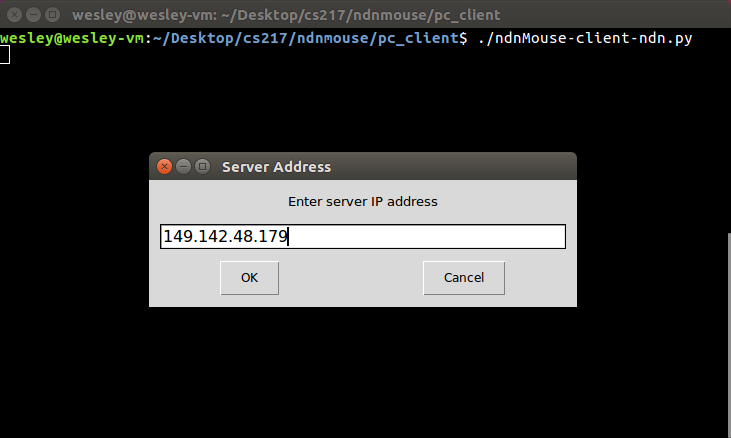
\includegraphics[width=11cm]{screenshots/client1}
\end{figure}

\begin{figure}[ht]
	\hypertarget{fig:client2}{}
	\centering
	\caption{PC program password entry}
	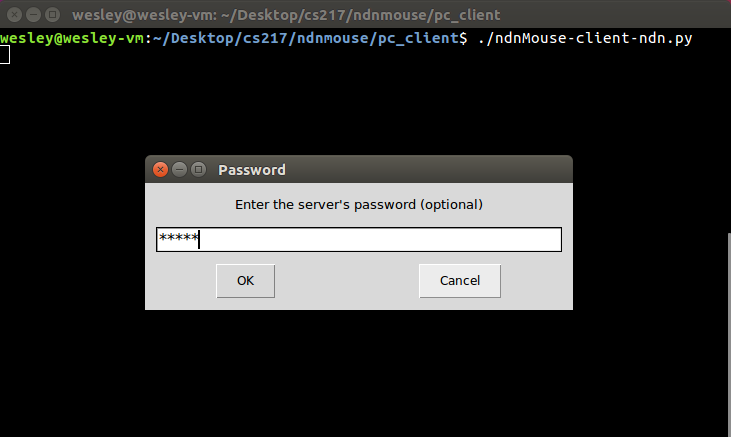
\includegraphics[width=11cm]{screenshots/client2}
\end{figure}

\begin{figure}[ht]
	\hypertarget{fig:client3}{}
	\centering
	\caption{PC program running}
	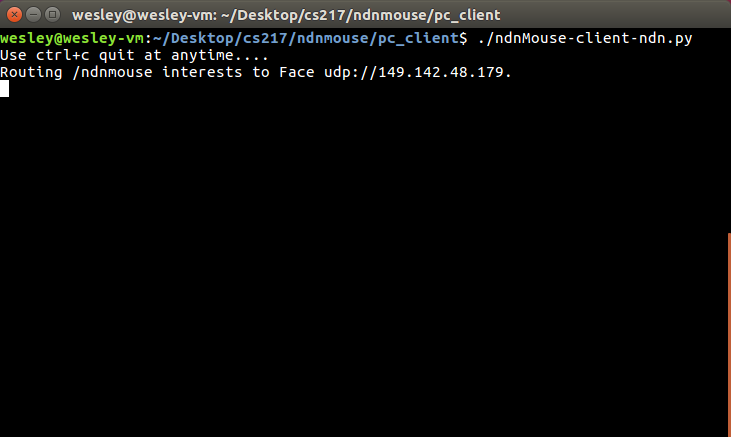
\includegraphics[width=11cm]{screenshots/client3}
\end{figure}

\end{document}